%Este trabalho está licenciado sob a Licença Atribuição-CompartilhaIgual 4.0 Internacional Creative Commons. Para visualizar uma cópia desta licença, visite http://creativecommons.org/licenses/by-sa/4.0/deed.pt_BR ou mande uma carta para Creative Commons, PO Box 1866, Mountain View, CA 94042, USA.

\chapter{Sistema de equações não lineares}\label{cap_snl}
\thispagestyle{fancy}

Neste capítulo, discutiremos sobre métodos para a resolução de sistema de equações não lineares. Vamos trata o caso de problemas da forma: encontrar $\pmb{x}\in\mathbb{R}^n$ tal que
\begin{equation}
  F(\pmb{x}) = \pmb{0},
\end{equation}
onde $F:\mathbb{R}^n\to\mathbb{R}^n$ é uma função vetorial dada.

\section{Método de Newton}\label{cap_snl_sec_newton}

Consideremos o problema de encontrar $\pmb{x} = (x_1, x_2, \dotsc, x_n)\in\mathbb{R}^n$ tal que
\begin{equation}
  F(\pmb{x}) = \pmb{0},
\end{equation}
onde $F:\mathbb{R}^n\to\mathbb{R}^n$ é uma função vetorial dada com $F(\pmb{x}) = (f_1(\pmb{x}), f_2(\pmb{x}), \dotsc, f_n(\pmb{x}))$. Suponhamos, então, que $\pmb{x}^*$ seja a solução exata deste problema e que $\pmb{x}^{(1)}$ seja uma aproximação de $\pmb{x}^*$. Assim sendo, tomemos a seguinte expansão de $F$ em polinômio de Taylor:
\begin{equation}
  F(\pmb{x}^*) = F(\pmb{x}^{(1)}) + J_F(\pmb{x}^{(1)})(\pmb{x}^*-\pmb{x}^{(1)}) + R,
\end{equation}
onde $J_F$ é a matriz jacobiana\footnote{Carl Gustav Jacob Jacobi, 1804 - 1851, matemático alemão. Fonte: \href{https://en.wikipedia.org/wiki/Carl_Gustav_Jacob_Jacobi}{Wikipedia}.} de $F$
\begin{equation}
  J_F :=
  \begin{bmatrix}
    \frac{\p f_1}{\p x_1} & \frac{\p f_1}{\p x_2} & \ldots & \frac{\p f_1}{\p x_n}\\
    \frac{\p f_2}{\p x_1} & \frac{\p f_2}{\p x_2} & \ldots & \frac{\p f_2}{\p x_n}\\
    \vdots & \vdots & \vdots & \vdots \\
    \frac{\p f_n}{\p x_1} & \frac{\p f_n}{\p x_2} & \ldots & \frac{\p f_n}{\p x_n}\\
  \end{bmatrix}
\end{equation}
e $\|R\|^2\to 0$ com $\|\pmb{x}^{(1)}-\pmb{x}^*\|\to 0$. 

Daí, como $F(\pmb{x}^*) = \pmb{0}$, temos
\begin{equation}
  J_F(\pmb{x}^{(1)})(\pmb{x}^*-\pmb{x}^{(1)}) \approx -F(\pmb{x}^{(1)}).
\end{equation}
Então, multiplicando a inversa da jacobiana à esquerda, obtemos
\begin{equation}
  \pmb{x}^*-\pmb{x}^{(1)} \approx - J_F^{-1}(\pmb{x}^{(1)})F(\pmb{x}^{(1)})
\end{equation}
e também
\begin{equation}
  \pmb{x}^* \approx \pmb{x}^{(1)} - J_F^{-1}(\pmb{x}^{(1)})F(\pmb{x}^{(1)}).
\end{equation}

O exposto acima nos motiva a \emph{iteração de Newton}\footnote{Sir Isaac Newton, 1642 - 1726/27, matemático e físico inglês. Fonte: \href{https://en.wikipedia.org/wiki/Isaac_Newton}{Wikipedia}.}:
\begin{align}
  \pmb{x}^{(1)} &= \text{aprox. inicial},\\
  \pmb{x}^{(k+1)} &= \pmb{x}^{(k)} - J_F^{-1}(\pmb{x}^{(k)})F(\pmb{x}^{(k)}),
\end{align}
com $k=1, 2, \ldots$.

\begin{ex}\label{ex:newton_intro}
  Consideremos o seguinte sistema de equações não lineares
  \begin{align}
    x_1x_2^2 &= x_1^2x_2 - 6,\\
    x_1^2x_2^3 - 7 &= -x_1.
  \end{align}
  Para usarmos o método de Newton, reescrevemos o sistema na seguinte forma
  \begin{align}
    x_1x_2^2 - x_1^2x_2 + 6 &= 0,\\
    x_1 + x_1^2x_2^3 - 7 &= 0.
  \end{align}
  Com isso, identificamos a função objetivo
  \begin{equation}
    F(\pmb{x}) =
    \begin{bmatrix}
      f_1(\pmb{x})\\
      f_2(\pmb{x})
    \end{bmatrix}
=
    \begin{bmatrix}
      x_1x_2^2 - x_1^2x_2 + 6\\
      x_1 + x_1^2x_2^3 - 7
    \end{bmatrix}
  \end{equation}
  e sua matriz jacobiana
  \begin{align}
    J_F(\pmb{x}) &= \frac{\p(f_1, f_2)}{\p(x_1, x_2)} =
          \begin{bmatrix}
            \frac{\p f_1}{\p x_1} & \frac{\p f_1}{\p x_2}\\
            \frac{\p f_2}{\p x_1} & \frac{\p f_2}{\p x_2}\\
          \end{bmatrix}\\
    &=
      \begin{bmatrix}
        x_2^2 - 2x_1x_2 & 2x_1x_2-x_1^2\\
        1+2x_1x_2^3 & 3x_1^2x_2^2
      \end{bmatrix}
  \end{align}
  Definidas $F$ e $J_F$ e tomando $\pmb{x}^{(1)} = (1,5,~1,5)$ como aproximação inicial, computamos as iterações de Newton de forma a obtermos os resultados apresentados na Tabela \ref{tab:newton_intro}.

  \begin{table}[h!]
    \centering
    \begin{tabular}{lcc}
      k & $\pmb{x}^{(k)}$ & $\|F(\pmb{x}^{(k)})\|$\\\hline
      1 & $(-1,50,~1,50)$ & $1,2\E+0$\\
      2 & $(-1,07,~1,82)$ & $1,2\E+0$\\
      3 & $(-9,95\E-1,~2,00)$ & $7,6\E-2$\\
      4 & $(-1,00,~2,00)$ & $1,2\E-4$ \\
      5 & $(-1,00,~2,00)$ & $2,1\E-9$ \\\hline
    \end{tabular}
    \caption{Resultados referentes ao Exemplo \ref{ex:newton_intro}.}
    \label{tab:newton_intro}
  \end{table}

\ifisoctave
No \verb+GNU Octave+, podemos fazer as computações acima com o seguinte \href{https://github.com/phkonzen/notas/blob/master/src/MatematicaNumerica/cap_snl/dados/ex_newton_intro/ex_newton_intro.m}{código}:
\verbatiminput{./cap_snl/dados/ex_newton_intro/ex_newton_intro.m}
\fi
\end{ex}

\subsection{Considerações sobre convergência}

Para uma função $F$ suficientemente suave e com uma escolha apropriada da aproximação inicial $\pmb{x}^{(1)}$, temos que as iterações de Newton
\begin{equation}
  \pmb{x}^{(k+1)} = \pmb{x}^{(k)} - J_F^{-1}(\pmb{x}^{(1)})F(\pmb{x}^{(1)}),
\end{equation}
são quadraticamente convergentes, i.e.
\begin{equation}
  \|\pmb{x}^{(k+1)} - \pmb{x}^*\| \leq C\|\pmb{x}^{(k)}-\pmb{x}^*\|^2,
\end{equation}
onde $\pmb{x}^*$ é a solução exata, i.e. $F(\pmb{x}^*) = \pmb{0}$.

\begin{ex}\label{ex:newton_conv}
  Consideremos o seguinte sistema de equações não lineares
  \begin{align}
    x_1x_2^2 - x_1^2x_2 + 6 &= 0,\\
    x_1 + x_1^2x_2^3 - 7 &= 0.
  \end{align}
  A Figura \ref{fig:ex_newton_conv} é um esboço do gráfico da $\|F(\cdot)\|$. Este problema foi confeccionado de forma que $\pmb{x}^* = (-1,~2)$. Então, tomando $\pmb{x}^{(1)} = (1,5,~1,5)$ como aproximação inicial, computamos as iterações de Newton para este problema, donde obtemos os resultados reportados na Tabela \ref{tab:ex_newton_conv}. 

  \begin{figure}[h!]
    \centering
    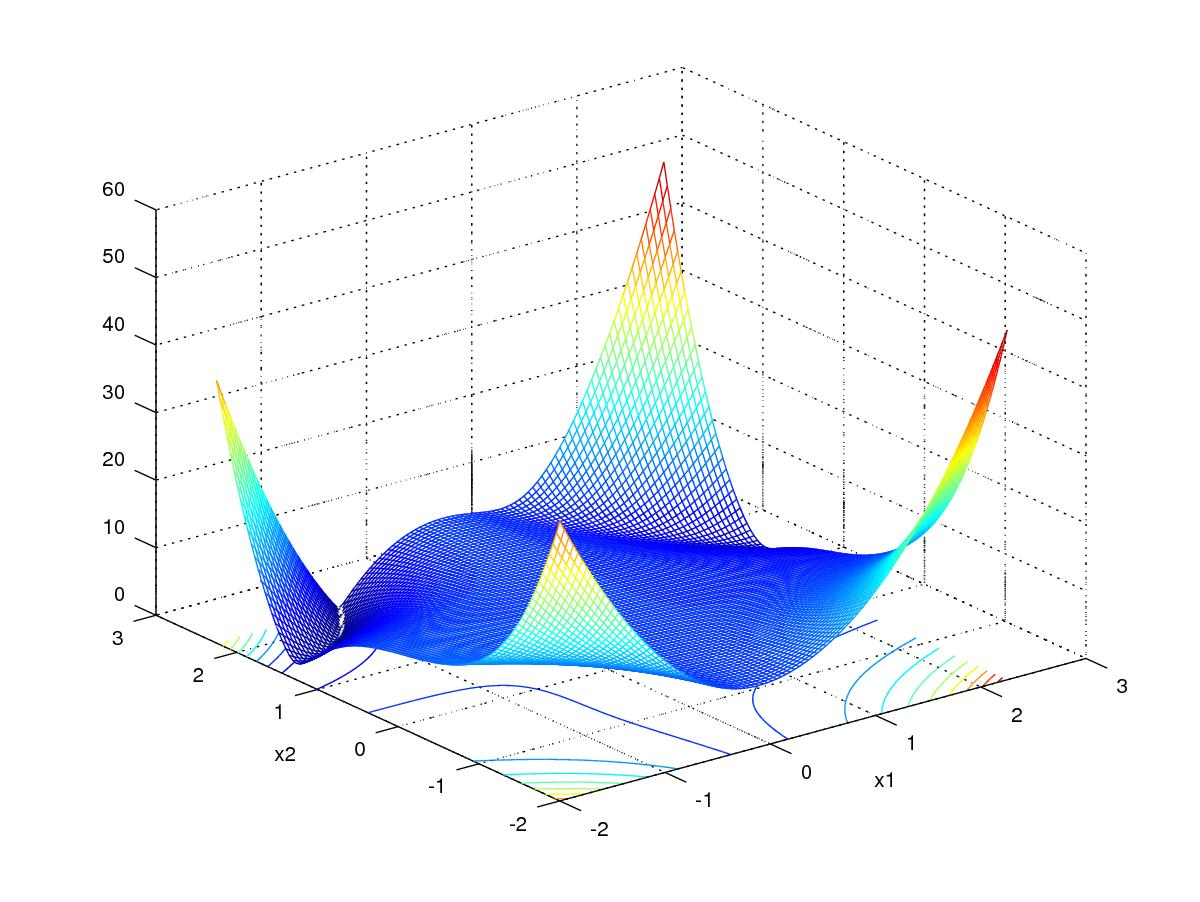
\includegraphics[width=0.7\textwidth]{./cap_snl/dados/ex_newton_conv/ex_newton_conv}
    \caption{Esboço do gráfico de $\|F(\cdot)\|$ referente ao Exemplo \ref{ex:newton_conv}.}
    \label{fig:ex_newton_conv}
  \end{figure}

  \begin{table}[h!]
    \centering
    \begin{tabular}{lcc}
      k & $\pmb{x}^{(k)}$ & $\|\pmb{x}^{(k)} - \pmb{x}^*\|$\\\hline
      1 & $(-1,50,~1,50)$ & $7,1\E-01$\\
      2 & $(-1,07,~1,82)$ & $2,0\E-01$\\
      3 & $(-9,95\E-1,~2,00)$ & $5,1\E-03$\\
      4 & $(-1,00,~2,00)$ & $2,6\E-05$ \\
      5 & $(-1,00,~2,00)$ & $2,0\E-10$ \\\hline
    \end{tabular}
    \caption{Resultados referentes ao Exemplo \ref{ex:newton_conv}.}
    \label{tab:ex_newton_conv}
  \end{table}

\ifisoctave
No \verb+GNU Octave+, podemos fazer as computações acima com o seguinte \href{https://github.com/phkonzen/notas/blob/master/src/MatematicaNumerica/cap_snl/dados/ex_newton_conv/ex_newton_conv.m}{código}:
\verbatiminput{./cap_snl/dados/ex_newton_conv/ex_newton_conv.m}
\fi
\end{ex}

\subsection*{Exercícios}

\begin{exer}\label{ex:newton_exec}
  Use o método de Newton para obter uma aproximação de uma solução de
  \begin{align}
    x_2\sen(x_3)+x_1-2&=0,\\
    x_1x_2-\sen(x_2)+0,2&=0,\\
    x_3^2+\cos(x_1x_2)-4,5&=0.
  \end{align}
Para tanto, use $\pmb{x}^{(1)} = (1,~-1,~-1)$.
\end{exer}
\begin{resp}
    \ifisoctave 
    \href{https://github.com/phkonzen/notas/blob/master/src/MatematicaNumerica/cap_snl/dados/exer_newton_exec/exer_newton_exec.m}{Código}. 
  \fi
  $x_1 = 1,7519\E+0$, $x_2 = -2,6202\E-1$, $x_3 =-1,8983\E+0$
\end{resp}



\section{Métodos {\it quasi}-Newton}\label{cap_snl_sec_quasi_newton}

\subsection{Método do acorde}

O método do acorde consiste na seguinte iteração
\begin{align}
  \pmb{x}^{(1)} &= \text{aprox. inicial},\\
  \pmb{x}^{(k+1)} &= \pmb{x}^{(k)} - J_F^{-1}(\pmb{x}^{(1)})F(\pmb{x}^{(k)}).
\end{align}
Ou seja, é a iteração de Newton com jacobina constante.

\begin{ex}\label{ex:acorde_exec}
  Consideremos o seguinte sistema de equações não lineares
  \begin{align}
    x_1x_2^2 - x_1^2x_2 + 6 &= 0,\\
    x_1 + x_1^2x_2^3 - 7 &= 0.
  \end{align}
  Definidas $F$ e $J_F$ e tomando $\pmb{x}^{(1)} = (1,5,~1,5)$ como aproximação inicial, computamos as iterações do método do acorde de forma a obtermos os resultados apresentados na Tabela \ref{tab:ex_acorde_exec}.

  \begin{table}[h!]
    \centering
    \begin{tabular}{lcc}
      k & $\pmb{x}^{(k)}$ & $\|\pmb{x}^{(k)} - \pmb{x}^*\|$\\\hline
      1 & $(-1,50,~1,50)$ & -x- \\
      2 & $(-1,07,~1.82)$ & $5,3\E-1$ \\
      3 & $(-1,02,~1,93)$ & $1,2\E-1$ \\
      4 & $(-1,00,~1,98)$ & $5,2\E-2$ \\
      5 & $(-9,98\E-1,~2,00)$ & $1,8\E-2$ \\
      6 & $(-9,98\E-1,~2,00)$ & $4,7\E-3$ \\
      7 & $(-9,99\E-1,~2,00)$ & $9,0\E-4$ \\
      8 & $(-1,00,~2,00)$ & $7,4\E-4$ \\
      9 & $(-1,00,~2,00)$ & $4,3\E-4$ \\\hline
    \end{tabular}
    \caption{Resultados referentes ao Exemplo \ref{ex:acorde_exec}.}
    \label{tab:ex_acorde_exec}
  \end{table}

\ifisoctave
No \verb+GNU Octave+, podemos fazer as computações acima com o seguinte \href{https://github.com/phkonzen/notas/blob/master/src/MatematicaNumerica/cap_snl/dados/ex_acorde_exec/ex_acorde_exec.m}{código}:
\verbatiminput{./cap_snl/dados/ex_acorde_exec/ex_acorde_exec.m}
\fi
\end{ex}

\subsection{Jacobiana aproximada}

A jacobiana $J_F(\pmb{x})$ de uma dada função $F(\pmb{x}) = (f_1(\pmb{x}), f_2(\pmb{x}), \dotsc, f_n(\pmb{x}))$ é a matriz cujo elemento da $i$-ésima linha e $j$-ésima coluna é
\begin{equation}
  \frac{\p f_i}{\p x_j} = \lim_{h\to 0} \frac{f_i(\pmb{x}+\pmb{e}_jh) - f_i(\pmb{x})}{h},
\end{equation}
onde $\pmb{e}_j$ é o $j$-ésimo vetor da base canônica de $\mathbb{R}^n$, i.e. $\pmb{e}_j = (0, \dotsc, 0, 1, 0, \dotsc, 0)$ com $1$ na $j$-ésima posição.

Com isso, podemos computar uma jacobiana aproximada tomando
\begin{equation}
  \frac{\p f_i}{\p x_j} \approx \frac{f_i(\pmb{x}+\pmb{e}_jh) - f_i(\pmb{x})}{h},
\end{equation}
com $h$ suficientemente pequeno.

\begin{ex}\label{ex:jacaprox_exec}
  Consideremos o seguinte sistema de equações não lineares
  \begin{align}
    x_1x_2^2 - x_1^2x_2 + 6 &= 0,\\
    x_1 + x_1^2x_2^3 - 7 &= 0.
  \end{align}
  Definida $F$, sua jacobina aproximada $\tilde{J}_F$ e tomando $\pmb{x}^{(1)} = (1,5,~1,5)$ como aproximação inicial, computamos as iterações do {\it quasi}-método de forma a obtermos os resultados apresentados na Tabela \ref{tab:ex_jacaprox_exec}.

  \begin{table}[h!]
    \centering
    \begin{tabular}{lcc}
      k & $\pmb{x}^{(k)}$ & $\|\pmb{x}^{(k)} - \pmb{x}^*\|$\\\hline
      1 & $(-1,50,~1,50)$ & -x- \\
      2 & $(-1,07,~1,82)$ & $5,3\E-1$\\
      3 & $(-9,95\E-1,~2,00)$ & $2,0\E-1$\\
      4 & $(-1,00,~2,00)$ & $5,1\E-3$\\
      5 & $(-1,00,~2,00)$ & $2,6\E-5$\\\hline
    \end{tabular}
    \caption{Resultados referentes ao Exemplo \ref{ex:jacaprox_exec}.}
    \label{tab:ex_jacaprox_exec}
  \end{table}

\ifisoctave
No \verb+GNU Octave+, podemos fazer as computações acima com o seguinte \href{https://github.com/phkonzen/notas/blob/master/src/MatematicaNumerica/cap_snl/dados/ex_jacaprox_exec/ex_jacaprox_exec.m}{código}:
\verbatiminput{./cap_snl/dados/ex_jacaprox_exec/ex_jacaprox_exec.m}
\fi
\end{ex}

\subsection*{Exercícios}

\emconstrucao